
\documentclass[aspectratio=43]{beamer}
\usetheme{Madrid}

\usepackage{graphicx}
\usepackage[utf8]{inputenc}
\usepackage{hyperref}
\usepackage{listings}

\begin{document}
	
	\title{Introducción a las redes neuronales}   
	\subtitle{Aspectos del entrenamiento} 
	\author[J.I. Vasquez]{\textbf{Juan Irving Vásquez} \\jivg.org}
	\date{\today \copyright}
	\institute[jivg.org]{Centro de Innovación y Desarrollo Tecnológico en Cómputo \\ Instituto Politécnico Nacional}
	% logo de la universidad
	\titlegraphic{
\includegraphics[width=2cm]{ipn-cidetec}}
	\frame{\titlepage} 
	
	
	%%%%%%%%%%%%%%%%%%%%%%%%%%%%%%%%%%%%%%%%%%%%%%%%%%%%%%%%
	
	
	\section{Métricas de desempeño}
	
	\frame{
		\frametitle{Matriz de confusión}
		\framesubtitle{Ejemplo de conjunto de datos}
		\begin{figure}
			\centering
			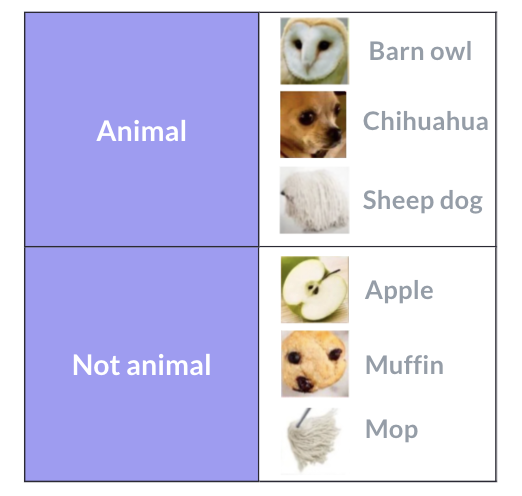
\includegraphics[height=0.65\textheight]{ds}
			\caption{Conjunto de datos de animales y no animales. \footnote{https://www.labelf.ai/blog/what-is-accuracy-precision-recall-and-f1-score}}
			\label{fig:ds}
		\end{figure}
	}    
	
	
	\begin{frame}
		\frametitle{Conceptos de predicción}
		\framesubtitle{Para clases binarias\footnote{Considera la clase 'animal' como la clase positiva.}}
		\centering
		\begin{tabular}{|c|c|c|}
			\hline
			Entrada de la red & Predicción & Concepto \\
			\hline
			
\includegraphics[width=0.1\textwidth]{chihuahua} & 'animal' & verdadero positivo (TP) \\
			
\includegraphics[width=0.1\textwidth]{chihuahua} & 'no animal' & falso negativo (FN) \\
			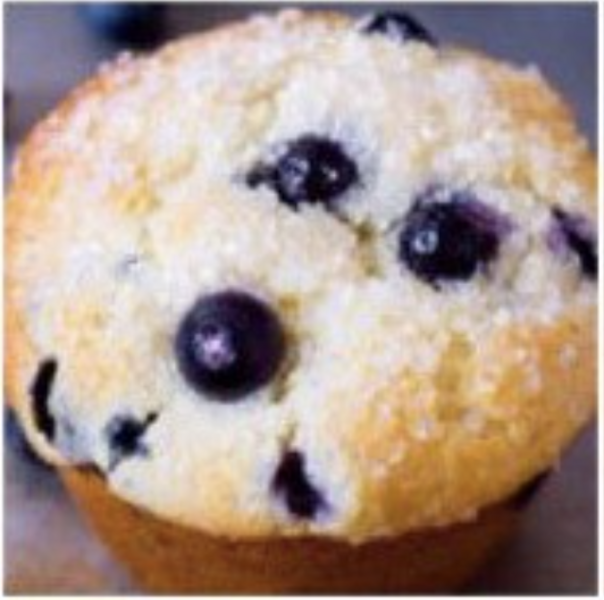
\includegraphics[width=0.1\textwidth]{muffin} & 'animal' & falso positivo (FP) \\
			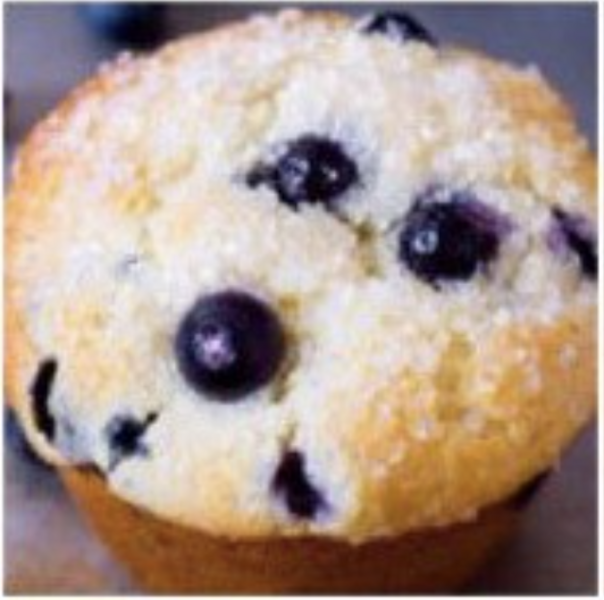
\includegraphics[width=0.1\textwidth]{muffin} & 'no animal' & verdadero negativo (TN) \\
			\hline
		\end{tabular}
	\end{frame}
	
	
	
	\frame{
		\frametitle{Matriz de confusión}
		\begin{itemize}
			\item Cálculo:
			\begin{table}
				\begin{tabular}{|c|c|c|}
					\hline
					Valor real & \textbf{Predicción positiva} & \textbf{Predicción negativa} \\ \hline
					\textbf{Clase positiva} & TP & FN \\ \hline
					\textbf{Clase negativa} & FP & TN \\ \hline
				\end{tabular}
				\caption{Matriz de confusión}
			\end{table}
			\item TP + FN suman el 100 \% de la clase positiva
			\item FP + TN suman el 100 \% de la clase negativa
		\end{itemize}
	}
	
	
	
	\frame{
		\frametitle{Ejercicio}
		\begin{figure}
			\centering
			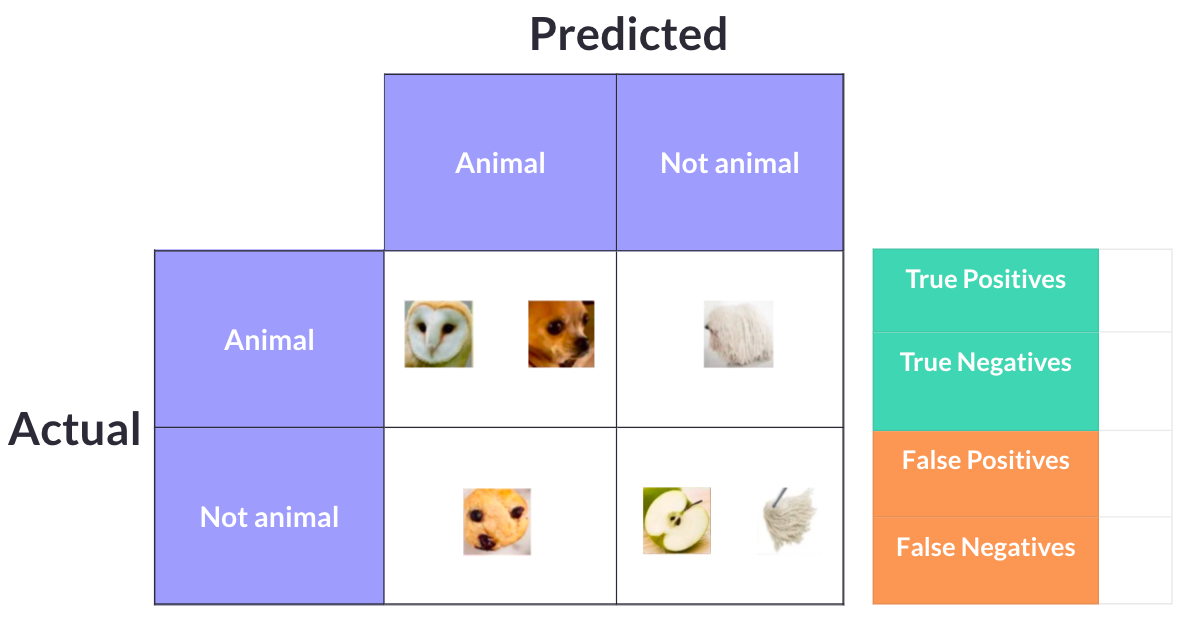
\includegraphics[height=0.7\textheight]{mc1}
			\caption{Ejemplo de matriz de confusión.}
			\label{fig:mc1}
		\end{figure}
	}
	
	\frame{
		\frametitle{Solución}
		\begin{figure}
			\centering
			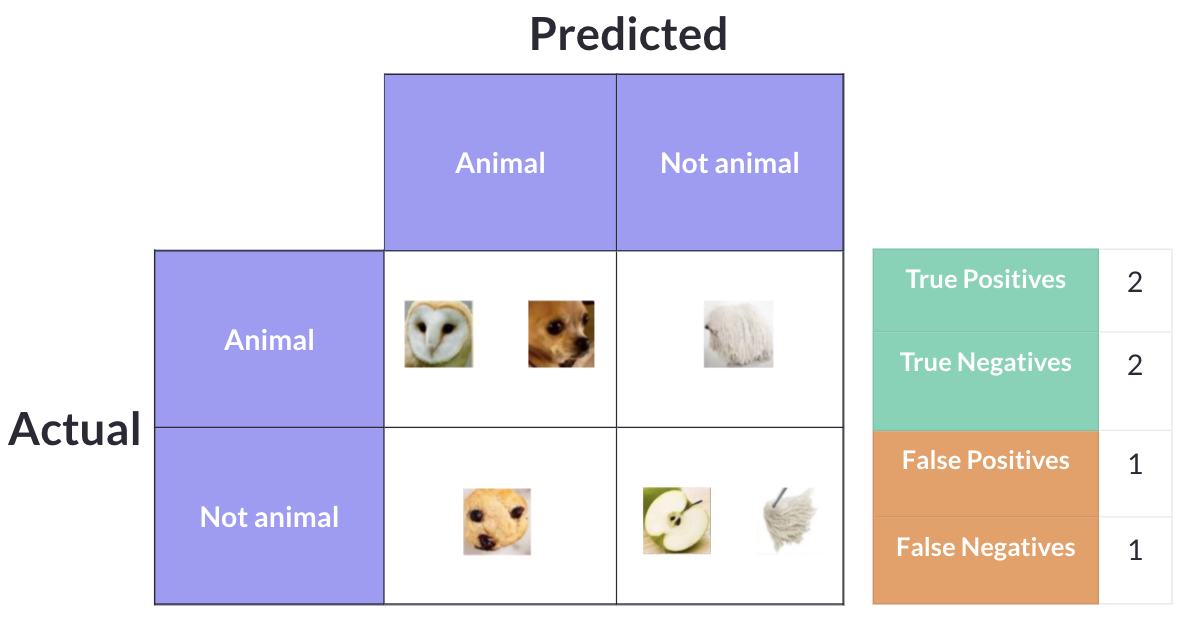
\includegraphics[height=0.7\textheight]{mc2}
			\caption{Ejemplo de matriz de confusión.}
			\label{fig:mc1}
		\end{figure}
	}
	
	
	
\end{document}
